% =====================================================================
% Bien dich bang XeLaTeX (khuyen nghi) hoac LuaLaTeX de ho tro Unicode
% tieng Viet day du:
%   xelatex bao_cao_hawkbot.tex
%   xelatex bao_cao_hawkbot.tex   (chay 2 lan de cap nhat muc luc/tham chieu)
% Neu khong co font "Noto Serif"/"Noto Sans", may tinh se tu dong dung
% font he thong thay the (fontspec se bao loi neu thieu hoan toan font
% Unicode -- khi do doi sang "DejaVu Serif" hoac "Times New Roman").
% =====================================================================
\documentclass[12pt,a4paper]{article}

\usepackage{fontspec}
\usepackage{polyglossia}
\setmainlanguage{vietnamese}
\setmainfont{Noto Serif}
\setsansfont{Noto Sans}
\setmonofont{Noto Sans Mono}

\usepackage[margin=2.5cm]{geometry}
\usepackage{graphicx}
\usepackage{booktabs}
\usepackage{multirow}
\usepackage{amsmath}
\usepackage{amssymb}
\usepackage{siunitx}
\usepackage{caption}
\usepackage{subcaption}
\usepackage{xcolor}
\usepackage{hyperref}
\usepackage{float}
\usepackage{enumitem}
\usepackage{algorithm}
\usepackage{algpseudocode}

\hypersetup{
    colorlinks=true,
    linkcolor=blue!50!black,
    citecolor=blue!50!black,
    urlcolor=blue!50!black
}

\sisetup{output-decimal-marker={,}, group-separator={.}}

\title{\textbf{Định vị vật thể tuyệt đối trong bản đồ ba chiều ngữ nghĩa\\
cho robot giao hàng tự hành: kết hợp hướng từ cụm điểm ngữ nghĩa\\
và khoảng cách đơn-ảnh}}
\author{Nhóm nghiên cứu Hawkbot}
\date{\today}

\begin{document}
\maketitle

\begin{abstract}
Bài báo trình bày một hệ thống dựng bản đồ ba chiều (3D) có gắn nhãn ngữ nghĩa cho robot giao hàng tự hành hoạt động trong nhà, kết hợp mô hình phát hiện đối tượng YOLO11n, mô hình tái tạo cảnh quan đơn mắt (monocular reconstruction) MapAnything, và một phương pháp định vị tuyệt đối vị trí đối tượng kết hợp hai tín hiệu độc lập. Tín hiệu thứ nhất là \emph{hướng} (bearing), xác định từ cụm điểm ngữ nghĩa lớn nhất tương ứng với đối tượng mục tiêu trong bản đồ điểm MapAnything (phân cụm bằng DBSCAN trên các điểm đã gán nhãn lớp), quy đổi sang hệ toạ độ thực bằng một phép khớp toàn cục (Umeyama fit — tỉ lệ, phép xoay, phép tịnh tiến) giữa quỹ đạo camera nội tại của MapAnything và quỹ đạo định vị hành trình (odometry) của robot, tính một lần cho toàn bộ phiên chụp. Tín hiệu thứ hai là \emph{khoảng cách}, ước lượng đơn-ảnh (monocular) từ kích thước khung bao (bounding box) phát hiện được trên một khung hình duy nhất, kết hợp chiều cao thật đã biết của đối tượng và tiêu cự camera đã hiệu chỉnh — hoàn toàn không phụ thuộc dữ liệu odometry. Phương pháp được xác thực trên sáu phiên chụp độc lập, mỗi lần robot quan sát cùng một đối tượng mục tiêu (một chậu cây cố định) theo một quỹ đạo di chuyển khác nhau: kết quả định vị dao động trong khoảng \SIrange{2.76}{3.26}{\meter} (trung bình \SI{3.02}{\meter}, độ lệch chuẩn \SI{0.19}{\meter}), khớp sát với giá trị đo thực địa bằng thước dây (\SI{3.00}{\meter}), sai số trung bình khoảng $6\%$. Đặc điểm cốt lõi giúp phương pháp ổn định qua nhiều lần lặp lại là: không có bước nào trong quy trình định vị đòi hỏi pose (vị trí và hướng) của một khung hình đơn lẻ phải chính xác tuyệt đối — hướng được suy ra từ một phép khớp toàn cục ít nhạy cảm với nhiễu cục bộ ở một vài khung hình, còn khoảng cách hoàn toàn tách biệt khỏi odometry. Bài báo cũng phân tích các giới hạn phần cứng hiện tại của nền tảng (độ phân giải camera thấp, năng lực tính toán tại biên hạn chế) làm cơ sở cho các lựa chọn thiết kế phương pháp, cùng các hướng phát triển tiếp theo.
\end{abstract}

\tableofcontents

% =====================================================================
\section{Giới thiệu}
% =====================================================================

Robot giao hàng tự hành hoạt động trong nhà cần xây dựng và duy trì một bản đồ ba chiều có gắn nhãn ngữ nghĩa (semantic 3D map) nhằm nhận biết vị trí các đối tượng và mốc tham chiếu trong môi trường — ví dụ hàng hoá cần giao, hoặc các vật thể cố định như chậu cây, bàn ghế, dùng làm điểm neo cho việc điều hướng. Một pipeline xử lý điển hình cho bài toán này kết hợp ba thành phần: (i) một mô hình phát hiện đối tượng hai chiều (YOLO) chạy trên từng khung hình camera, (ii) một mô hình tái tạo cảnh quan ba chiều từ ảnh đơn mắt (monocular 3D reconstruction) để khôi phục hình học của không gian, và (iii) một cơ chế xác định vị trí tuyệt đối của đối tượng trong hệ toạ độ thực (đơn vị mét), thường dựa trên dữ liệu định vị hành trình (odometry) của robot.

Việc triển khai một hệ thống định vị đối tượng trong điều kiện thực tế — sử dụng phần cứng chi phí thấp và dữ liệu định vị hành trình (odometry) vốn tích luỹ sai số theo thời gian — đặt ra câu hỏi cốt lõi về việc đâu là yếu tố thực sự chi phối độ chính xác của hệ thống, và làm thế nào để cải thiện độ tin cậy một cách hiệu quả nhất trong giới hạn tài nguyên hiện có. Trong quá trình triển khai thực nghiệm trên nền tảng robot Hawkbot (vận hành trên ROS2 Jazzy) với camera ESP32-CAM, nhóm nghiên cứu nhận thấy rằng các phương pháp định vị phụ thuộc trực tiếp vào pose (vị trí và hướng) odometry của \emph{từng khung hình riêng lẻ} rất nhạy với nhiễu cục bộ. Bài báo này trình bày một phương pháp định vị thay thế, kết hợp \textbf{hướng} suy ra từ cụm điểm ngữ nghĩa của đối tượng trong bản đồ điểm MapAnything (quy đổi sang hệ toạ độ thực bằng một phép khớp toàn cục trên cả quỹ đạo, thay vì dựa vào một khung hình đơn lẻ) với \textbf{khoảng cách} ước lượng đơn-ảnh không phụ thuộc odometry. Phương pháp được xác thực bằng số đo thực địa qua sáu phiên chụp độc lập, cho kết quả ổn định và nhất quán, mở ra một hướng thiết kế pipeline định vị ít nhạy cảm hơn với nhiễu odometry cục bộ, không đòi hỏi đầu tư thêm phần cứng.

% =====================================================================
\section{Phương pháp}
% =====================================================================

\subsection{Nền tảng phần cứng}

\begin{table}[H]
\centering
\caption{Thông số kỹ thuật hệ thống}
\label{tab:hw-specs}
\begin{tabular}{@{}ll@{}}
\toprule
\textbf{Thành phần} & \textbf{Thông số} \\
\midrule
Robot & Hawkbot, điều khiển qua ROS2 Jazzy (container \texttt{hawkbot-bringup}) \\
Camera & ESP32-CAM, độ phân giải QVGA ($320\times240$ px) \\
Nguồn odometry & \texttt{nav\_msgs/Odometry} trên topic \texttt{/odom} \\
Máy tính xử lý & Máy chủ GPU từ xa, kết nối qua mạng nội bộ \\
Mô hình phát hiện & YOLO11n (nano), huấn luyện sẵn trên COCO-80 \\
Mô hình dựng 3D & MapAnything (\texttt{facebook/map-anything}, HuggingFace) \\
\bottomrule
\end{tabular}
\end{table}

\begin{table}[H]
\centering
\caption{Ma trận nội tại camera $K$ (hiệu chỉnh bằng phương pháp bàn cờ, 74/75 ảnh hợp lệ, sai số tái chiếu trung bình 0,12 điểm ảnh)}
\label{tab:intrinsics}
\[
K = \begin{bmatrix}
428{,}72 & 0 & 148{,}61 \\
0 & 427{,}60 & 126{,}02 \\
0 & 0 & 1
\end{bmatrix}
\]
\end{table}

\begin{figure}[H]
\centering

\includegraphics[width=0.85\textwidth]{paper_figs/anh_thuc_te.jpg}
\caption{Môi trường thử nghiệm thực tế: robot Hawkbot (đơn vị hình trụ nhỏ ở giữa sàn) hoạt động trong không gian văn phòng, với chậu cây làm đối tượng mục tiêu chính của các thực nghiệm trình bày trong bài báo này.}
\label{fig:real-photo}
\end{figure}

\subsection{Hạn chế của nền tảng phần cứng hiện tại}
\label{sec:hw-limits}

Trước khi trình bày kiến trúc pipeline, cần làm rõ hai giới hạn phần cứng có ảnh hưởng xuyên suốt đến các lựa chọn phương pháp luận của nghiên cứu này.

\textbf{Độ phân giải camera.} Camera ESP32-CAM được cấu hình ở độ phân giải QVGA ($320\times240$ điểm ảnh) nhằm đảm bảo băng thông truyền ảnh qua mạng không dây và tốc độ khung hình ổn định. Tuy nhiên, độ phân giải thấp này giới hạn đáng kể độ chính xác định vị góc (angular precision) của mọi phương pháp dựa trên việc xác định vị trí điểm ảnh — bao gồm cả tâm bounding box của YOLO lẫn các phương pháp thay thế đã được thử nghiệm. Cụ thể, khi đánh giá phương án dùng mã định vị ArUco kích thước \SI{15}{\centi\meter} làm điểm neo tuyệt đối (trình bày chi tiết ở Mục~\ref{sec:hw-alternatives}), một sai lệch một điểm ảnh trong việc xác định góc của mã, ở khoảng cách quan sát trên hai mét, đã tương ứng với sai số vị trí thực tế lên tới vài chục xăng-ti-mét. Đây là hệ quả trực tiếp của việc đối tượng mục tiêu chỉ chiếm một số lượng điểm ảnh rất nhỏ trong khung hình \num{320}$\times$\num{240}.

\textbf{Năng lực tính toán.} Camera ESP32-CAM không có khả năng xử lý thị giác máy tính tại chỗ (on-device inference); toàn bộ suy luận mô hình YOLO và MapAnything được thực hiện trên một máy chủ GPU từ xa, kết nối qua mạng cục bộ. Kiến trúc này kéo theo hai hệ quả: thứ nhất, pipeline hiện tại vận hành theo phương thức xử lý hậu kỳ (offline, post-hoc) trên toàn bộ phiên thu thập dữ liệu, chứ không phải một hệ thống định vị và dựng bản đồ đồng thời theo thời gian thực (real-time SLAM); thứ hai, việc bổ sung các cơ chế hiệu chỉnh trực tuyến — như đóng vòng lặp (loop closure) hoặc tối ưu hoá đồ thị tư thế toàn cục — vốn là giải pháp kỹ thuật chuẩn mực cho vấn đề trôi định vị, đòi hỏi đầu tư kỹ thuật và tài nguyên tính toán đáng kể mà nền tảng hiện tại chưa đáp ứng được.

Hai giới hạn trên là lý do trực tiếp khiến nghiên cứu này tập trung tìm kiếm một \textbf{giải pháp thuần phần mềm, không đòi hỏi nâng cấp phần cứng} — cụ thể là phương pháp kết hợp hướng từ cụm điểm ngữ nghĩa và khoảng cách đơn-ảnh trình bày ở Mục~\ref{sec:math} — thay vì theo đuổi các hướng khắc phục bằng phần cứng bổ sung (camera độ phân giải cao hơn, mã định vị lớn hơn, hoặc cụm tính toán biên mạnh hơn), vốn nằm ngoài phạm vi tài nguyên hiện có của dự án và được đề xuất là hướng phát triển trong tương lai (Mục~\ref{sec:limitations}).

\subsection{Kiến trúc pipeline}

Các bước xử lý được thực hiện tuần tự cho mỗi phiên chụp (capture) như sau:

\begin{enumerate}[label=\textbf{Bước \arabic*.}]
    \item \textbf{Thu thập dữ liệu:} Robot di chuyển tự do trong phòng, camera chụp ảnh liên tục ($\sim$1 khung/giây), đồng thời ghi lại vị trí và hướng (odometry) tương ứng từng khung hình vào \texttt{poses.json}.
    \item \textbf{Chọn khung hình ưu tiên:} Chạy YOLO trên toàn bộ khung hình gốc, ưu tiên chọn ra tối đa 130 khung có chứa đối tượng mục tiêu (chậu cây), lấy mẫu đều theo từng ``lần ghé qua'' (visit) để đảm bảo đa dạng góc nhìn.
    \item \textbf{Dựng phòng 3D:} Chạy MapAnything trên tập khung đã chọn, đồng thời gán nhãn lớp COCO (từ YOLO) cho từng điểm 3D, tạo ra một bản đồ điểm ngữ nghĩa của toàn bộ phòng và quỹ đạo camera riêng của MapAnything (trong hệ toạ độ nội tại của mô hình, không phải hệ toạ độ thực).
    \item \textbf{Khớp toàn cục với odometry:} Dùng phép khớp Umeyama giữa quỹ đạo camera của MapAnything và quỹ đạo odometry để tìm phép biến đổi (tỉ lệ $s$, phép xoay $R$, phép tịnh tiến $t$) quy đổi toàn bộ không gian của MapAnything sang hệ toạ độ thực — tính một lần cho cả phiên chụp, không phụ thuộc riêng một khung hình nào.
    \item \textbf{Xác định hướng đối tượng:} Lọc các điểm 3D mang nhãn lớp mục tiêu, phân cụm bằng DBSCAN, lấy tâm của cụm điểm lớn nhất; áp dụng phép khớp toàn cục ở bước trên để suy ra hướng (bearing) từ vị trí camera tham chiếu đến đối tượng trong không gian thực.
    \item \textbf{Xác định khoảng cách đối tượng:} Trên một khung hình duy nhất có phát hiện đối tượng, ước lượng khoảng cách đơn-ảnh từ chiều cao khung bao YOLO, chiều cao thật đã biết của đối tượng, và tiêu cự camera (\S~\ref{sec:math}) — độc lập hoàn toàn với odometry.
    \item \textbf{Kết hợp:} Vị trí đối tượng = vị trí camera tham chiếu + hướng $\times$ khoảng cách.
\end{enumerate}

Thuật toán~\ref{alg:labeling} mô tả chi tiết cơ chế gán nhãn ngữ nghĩa cho điểm 3D ở Bước~3 — bước nền tảng cho việc xác định cụm điểm mục tiêu ở Bước~5.

\begin{algorithm}[H]
\caption{Gán nhãn ngữ nghĩa cho đám mây điểm 3D}
\label{alg:labeling}
\begin{algorithmic}[1]
\Require Tập khung hình đã chọn $\{I_1, \dots, I_n\}$; mô hình MapAnything $\mathcal{M}$; mô hình YOLO $\mathcal{Y}$
\Ensure Đám mây điểm có nhãn $\mathcal{P} = \{(\mathbf{x}_j, l_j)\}$
\State $\mathcal{P} \gets \emptyset$
\For{$i \gets 1$ \textbf{to} $n$}
    \State $(D_i, K_i, T_i, M_i) \gets \mathcal{M}(I_i)$ \Comment{độ sâu, nội tại, pose camera, mặt nạ điểm hợp lệ}
    \State $\mathbf{P}_i \gets \textsc{DepthToWorld}(D_i, K_i, T_i)$ \Comment{toạ độ 3D cho từng pixel, kích thước $H \times W$}
    \State $B_i \gets \mathcal{Y}(I_i)$ \Comment{danh sách $(l, \text{bbox}, \text{conf})$ từ YOLO, đã lọc theo ngưỡng conf}
    \For{mỗi pixel $(u, v)$ với $M_i(u, v) = \text{true}$}
        \State $l \gets -1$ \Comment{mặc định: nền, không thuộc lớp nào}
        \For{mỗi $(l', \text{bbox}, \text{conf}) \in B_i$}
            \If{$(u, v) \in \text{bbox}$} \Comment{kiểm tra pixel nằm trong khung bao 2D}
                \State $l \gets l'$; \textbf{break}
            \EndIf
        \EndFor
        \State $\mathcal{P} \gets \mathcal{P} \cup \{(\mathbf{P}_i(u, v),\ l)\}$
    \EndFor
\EndFor
\State \Return $\mathcal{P}$
\end{algorithmic}
\end{algorithm}

\textbf{Lưu ý về hạn chế của cơ chế gán nhãn.} Phép kiểm tra ở dòng 8 (Thuật toán~\ref{alg:labeling}) chỉ xác định pixel có nằm trong \emph{khung chữ nhật} 2D của YOLO hay không — đây không phải một mô hình phân đoạn ngữ nghĩa (semantic segmentation) thực thụ ở cấp độ pixel. Do khung bao là hình chữ nhật bao quanh vật thể, các điểm nền hoặc vật thể khác nằm lọt vào bên trong khung bao (ví dụ khoảng trống phía sau đối tượng, hoặc mép của vật thể lân cận) cũng bị gán nhầm nhãn của đối tượng mục tiêu. Đây chính là lý do bước phân cụm DBSCAN ở Bước~5 là cần thiết: trong tập điểm đã gán nhãn (có lẫn nhiễu), cụm điểm dày đặc nhất — ứng với bản thân vật thể thật, được quan sát nhất quán từ nhiều góc nhìn — được tách ra khỏi các điểm nhiễu rải rác bị gán nhầm nhãn theo cơ chế hình chữ nhật này.

\subsection{Công thức}
\label{sec:math}

\textbf{Khớp toàn cục (Umeyama fit).} Gọi $\{\mathbf{q}_k\}$ là tập vị trí camera của MapAnything (chiếu xuống mặt phẳng ngang, hệ toạ độ nội tại) và $\{\mathbf{p}_k\}$ là vị trí odometry tương ứng của cùng các khung hình đó. Phép khớp Umeyama tìm tỉ lệ $s \in \mathbb{R}$, ma trận xoay $R \in SO(2)$ và véc-tơ tịnh tiến $\mathbf{t}$ tối thiểu hoá:
\begin{equation}
(s^*, R^*, \mathbf{t}^*) = \operatorname*{arg\,min}_{s, R, \mathbf{t}} \sum_k \left\lVert \mathbf{p}_k - \left(s R \mathbf{q}_k + \mathbf{t}\right) \right\rVert^2
\end{equation}
giải trực tiếp bằng phân tích SVD trên ma trận hiệp phương sai chéo giữa hai tập điểm đã căn giữa (centered). Một điểm bất kỳ $\mathbf{x}_{\text{raw}}$ trong không gian nội tại của MapAnything được quy đổi sang toạ độ thực bằng $\mathbf{x}_{\text{real}} = s^* R^* \mathbf{x}_{\text{raw}} + \mathbf{t}^*$.

\textbf{Hướng (bearing).} Gọi $\mathbf{c}_{\text{raw}}$ là tâm cụm điểm ngữ nghĩa lớn nhất (không gian nội tại MapAnything) và $\mathbf{o}$ là vị trí camera tham chiếu (hệ toạ độ thực, từ odometry). Hướng đơn vị:
\begin{equation}
\hat{\mathbf{b}} = \frac{\left(s^* R^* \mathbf{c}_{\text{raw}} + \mathbf{t}^*\right) - \mathbf{o}}{\left\lVert \left(s^* R^* \mathbf{c}_{\text{raw}} + \mathbf{t}^*\right) - \mathbf{o} \right\rVert}
\end{equation}

\textbf{Khoảng cách đơn-ảnh.} Với chiều cao khung bao YOLO $h_{\text{px}}$ (điểm ảnh) trên một khung hình, chiều cao thật đã biết $H$ (mét) của đối tượng, và tiêu cự camera $f_y$ (điểm ảnh, từ ma trận nội tại $K$, Bảng~\ref{tab:intrinsics}):
\begin{equation}
d = \frac{f_y \cdot H}{h_{\text{px}}}
\end{equation}

\textbf{Vị trí đối tượng cuối cùng:}
\begin{equation}
\mathbf{x}^* = \mathbf{o} + d \, \hat{\mathbf{b}}
\end{equation}

Không có đại lượng nào trong bốn công thức trên phụ thuộc vào pose odometry của một khung hình đơn lẻ ngoài vị trí camera tham chiếu $\mathbf{o}$ (dùng để neo kết quả, không ảnh hưởng đến hướng hay khoảng cách suy ra) — phép khớp toàn cục dùng toàn bộ quỹ đạo, còn khoảng cách hoàn toàn không dùng odometry.

% =====================================================================
\section{Kết quả thực nghiệm}
\label{sec:semantic-bearing}
% =====================================================================

Phương pháp định vị đối tượng trình bày ở Mục~\ref{sec:math} kết hợp hai tín hiệu độc lập:

\begin{itemize}
    \item \textbf{Hướng (bearing):} xác định từ cụm điểm ngữ nghĩa lớn nhất tương ứng với đối tượng mục tiêu trong bản đồ điểm MapAnything (phân cụm bằng DBSCAN trên các điểm đã gán nhãn lớp), quy đổi sang hệ toạ độ thực bằng một phép khớp toàn cục (Umeyama fit — tỉ lệ, phép xoay, phép tịnh tiến) giữa quỹ đạo camera nội tại của MapAnything và quỹ đạo odometry, tính một lần cho toàn bộ phiên chụp.
    \item \textbf{Khoảng cách:} ước lượng đơn-ảnh (monocular), tính trực tiếp từ chiều cao bounding box YOLO của một khung hình duy nhất, chiều cao thật đã biết của đối tượng, và tiêu cự camera đã hiệu chỉnh — không sử dụng dữ liệu odometry.
\end{itemize}

Vị trí cuối cùng của đối tượng được tính bằng vị trí camera tham chiếu cộng với tích của hướng và khoảng cách. Hình~\ref{fig:pipeline-new} minh hoạ toàn bộ pipeline.

\begin{figure}[H]
\centering
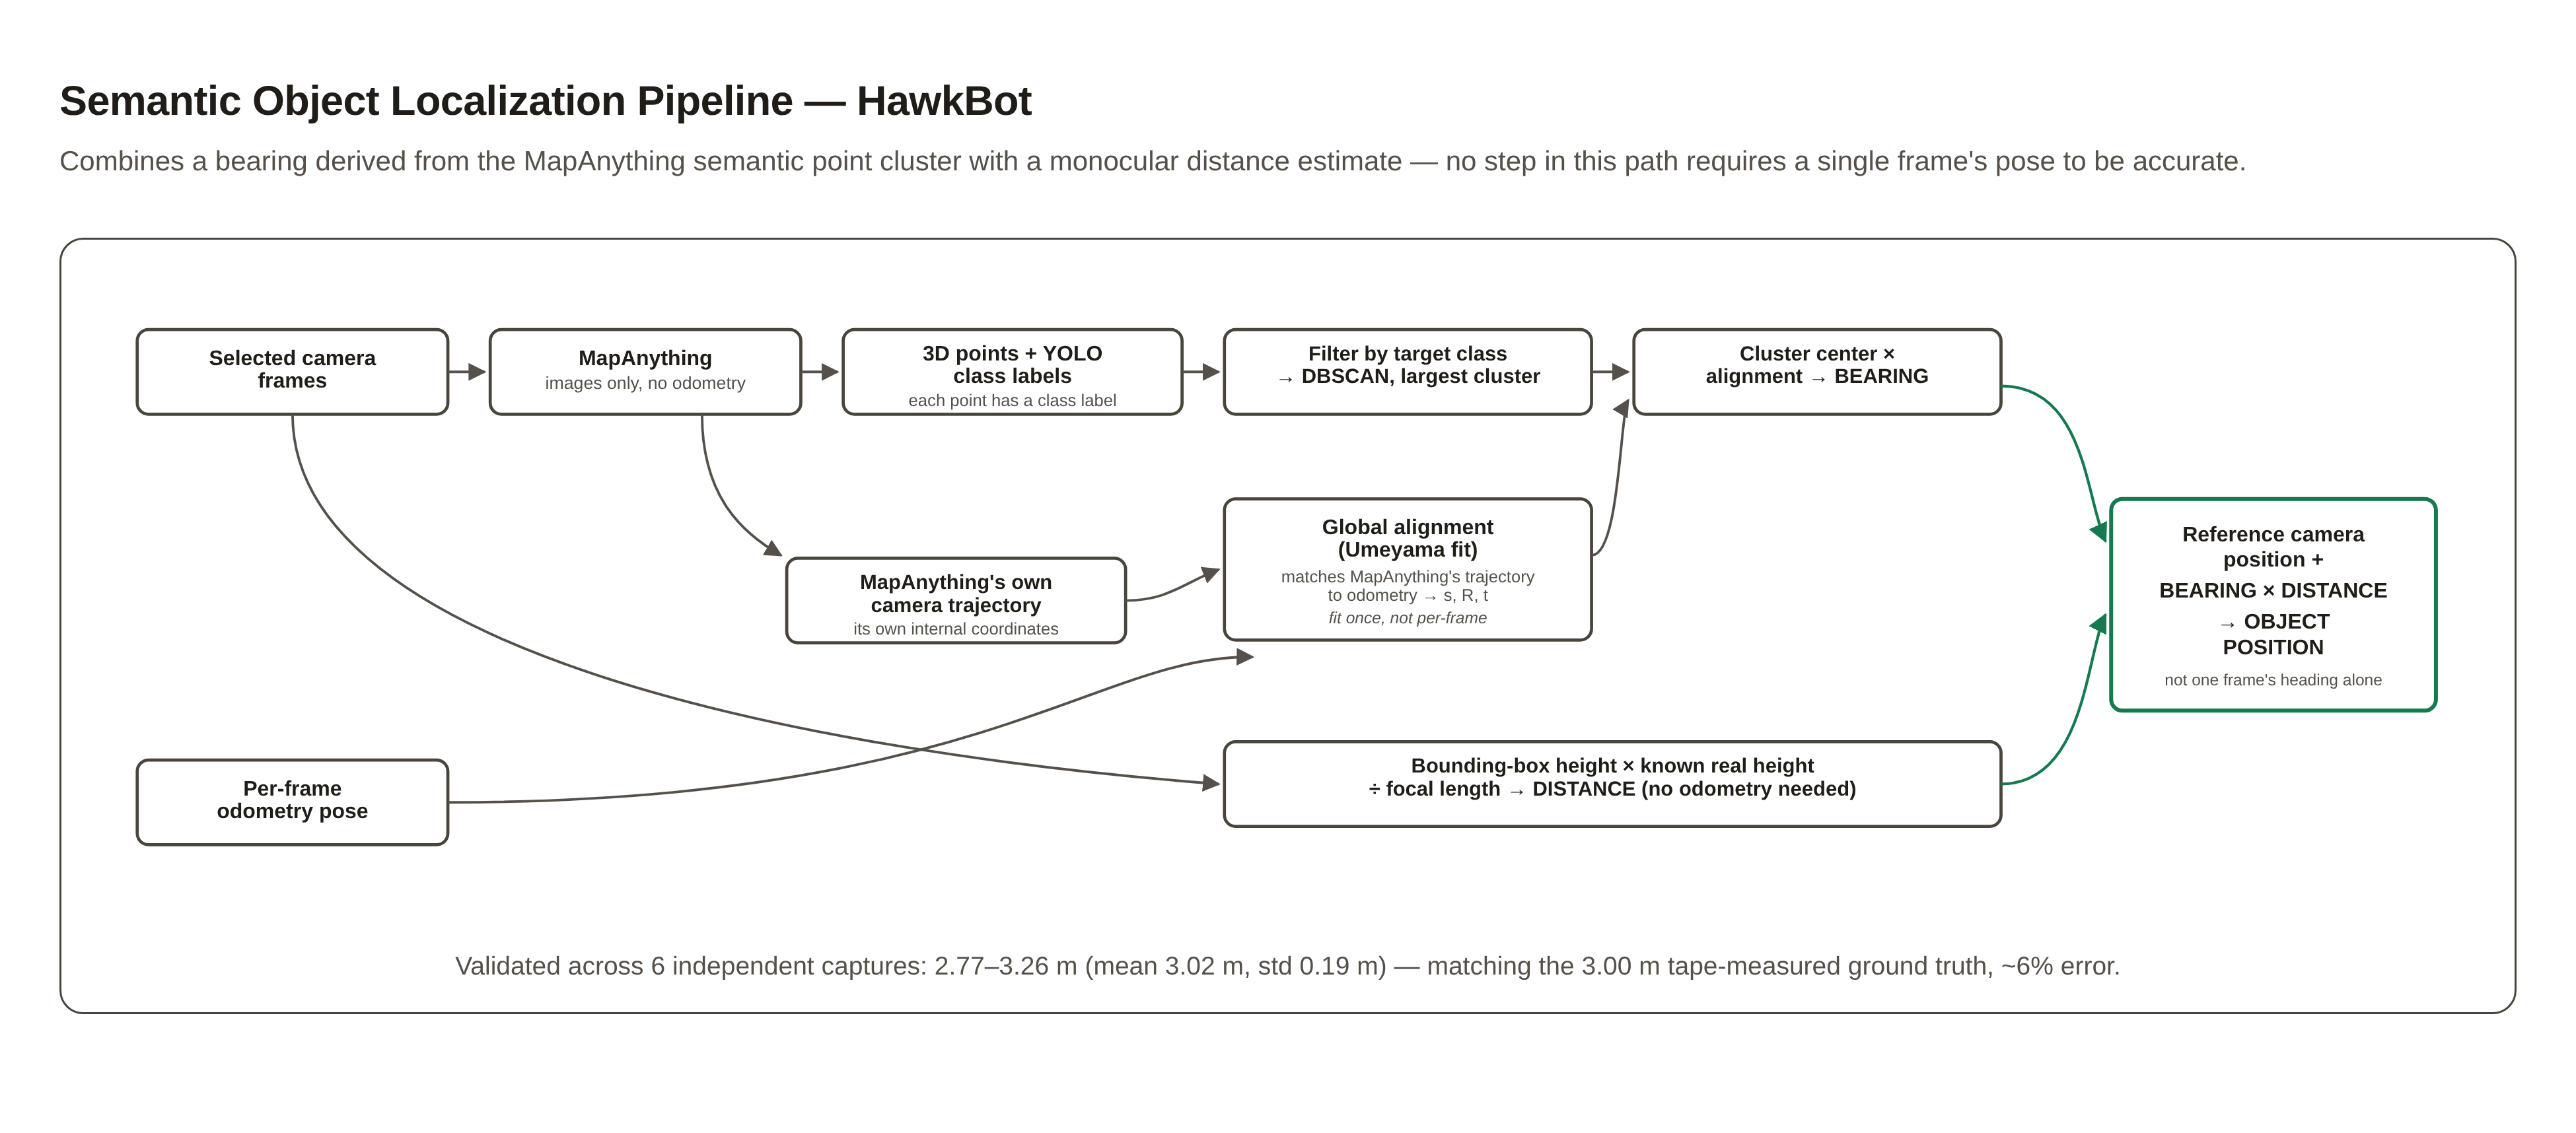
\includegraphics[width=\textwidth]{paper_figs/fig_pipeline_final.png}
\caption{Pipeline định vị đối tượng bằng hướng từ cụm điểm ngữ nghĩa MapAnything kết hợp khoảng cách đơn-ảnh.}
\label{fig:pipeline-new}
\end{figure}

Phương pháp được xác thực trên sáu phiên chụp độc lập (capture 36, 46--50), mỗi lần robot quan sát cùng một chậu cây theo một quỹ đạo di chuyển khác nhau. Bảng~\ref{tab:semantic-bearing-results} tổng hợp kết quả, đối chiếu với giá trị đo thực địa bằng thước dây.

\begin{table}[H]
\centering
\caption{Kết quả định vị chậu cây qua sáu phiên chụp độc lập}
\label{tab:semantic-bearing-results}
\begin{tabular}{@{}lc@{}}
\toprule
\textbf{Capture} & \textbf{Khoảng cách ước lượng} \\
\midrule
36 & \SI{2.77}{\meter} \\
46 & \SI{2.76}{\meter} \\
47 & \SI{3.13}{\meter} \\
48 & \SI{3.08}{\meter} \\
49 & \SI{3.26}{\meter} \\
50 & \SI{3.12}{\meter} \\
\midrule
Trung bình & \SI{3.02}{\meter} \\
Độ lệch chuẩn & \SI{0.19}{\meter} \\
\midrule
\multicolumn{2}{r}{\emph{Giá trị đo thực địa (thước dây):} \textbf{\SI{3.00}{\meter}}} \\
\bottomrule
\end{tabular}
\end{table}

Kết quả sáu lần đo hội tụ chặt quanh giá trị đo thực địa, sai số trung bình khoảng $6\%$. Hình~\ref{fig:six-viewers} minh hoạ vị trí đối tượng định vị được (marker xanh lá, kèm khoảng cách ước lượng) cùng quỹ đạo robot (đường đỏ) trên bản đồ điểm đám mây tương ứng của cả sáu phiên chụp.

\begin{figure}[H]
\centering
\begin{subfigure}[t]{0.32\textwidth}
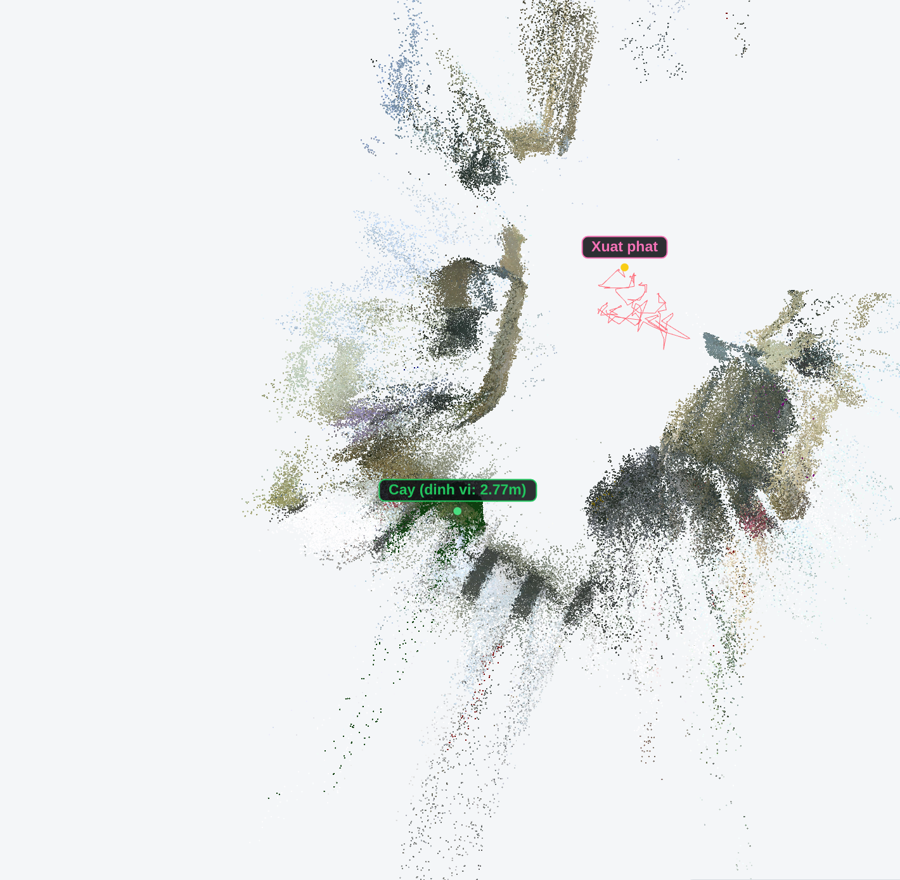
\includegraphics[width=\textwidth]{paper_figs/paperfig_new36.png}
\caption{Capture 36 — \SI{2.77}{\meter}}
\end{subfigure}
\hfill
\begin{subfigure}[t]{0.32\textwidth}
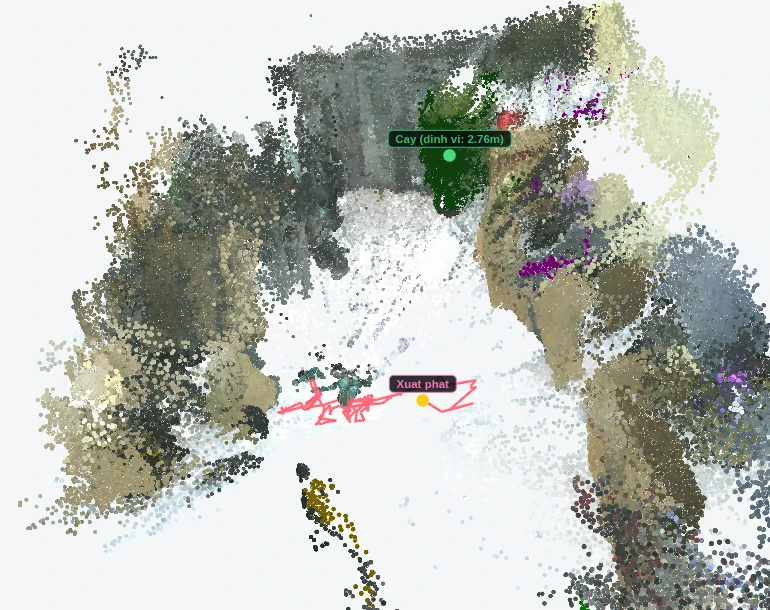
\includegraphics[width=\textwidth]{paper_figs/paperfig_new46.png}
\caption{Capture 46 — \SI{2.76}{\meter}}
\end{subfigure}
\hfill
\begin{subfigure}[t]{0.32\textwidth}
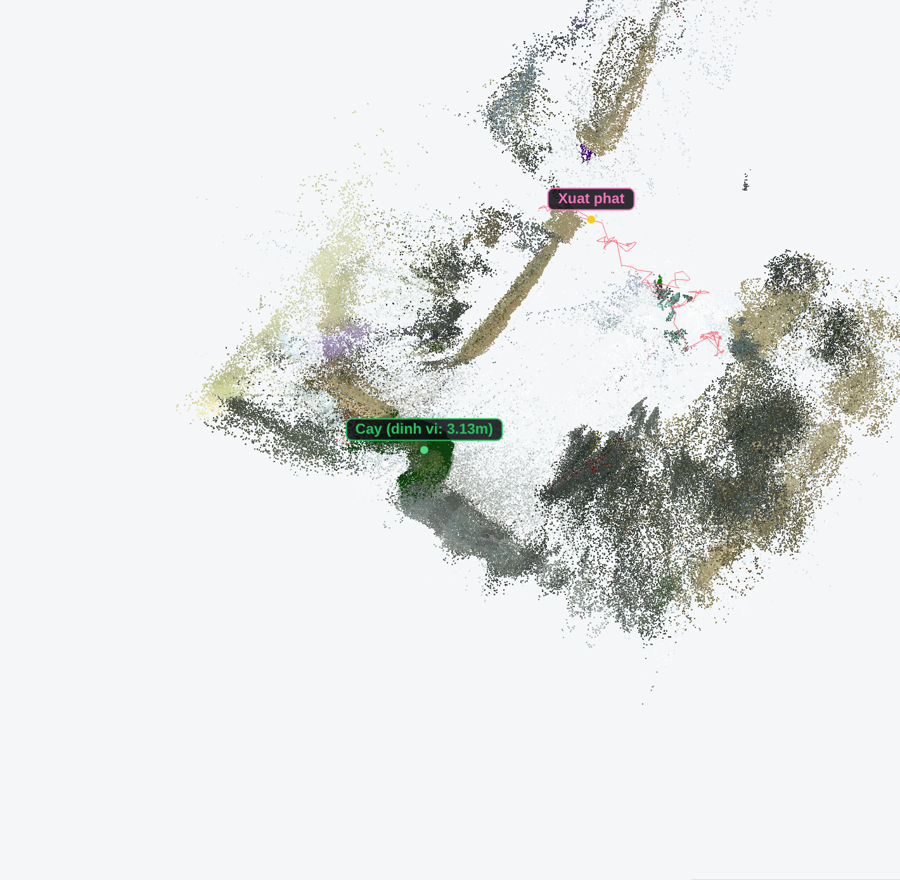
\includegraphics[width=\textwidth]{paper_figs/paperfig_new47.png}
\caption{Capture 47 — \SI{3.13}{\meter}}
\end{subfigure}

\vspace{0.6em}
\begin{subfigure}[t]{0.32\textwidth}

\includegraphics[width=\textwidth]{paper_figs/paperfig_new48.png}
\caption{Capture 48 — \SI{3.08}{\meter}}
\end{subfigure}
\hfill
\begin{subfigure}[t]{0.32\textwidth}

\includegraphics[width=\textwidth]{paper_figs/paperfig_new49.png}
\caption{Capture 49 — \SI{3.26}{\meter}}
\end{subfigure}
\hfill
\begin{subfigure}[t]{0.32\textwidth}

\includegraphics[width=\textwidth]{paper_figs/paperfig_new50.png}
\caption{Capture 50 — \SI{3.12}{\meter}}
\end{subfigure}
\caption{Vị trí chậu cây định vị được (marker xanh lá, nhãn ``Cây'') và quỹ đạo robot (đường đỏ, nhãn ``Xuất phát'' tại điểm bắt đầu) trên bản đồ điểm đám mây MapAnything, cho sáu phiên chụp độc lập.}
\label{fig:six-viewers}
\end{figure}

% =====================================================================
\section{Thảo luận}
% =====================================================================

\subsection{Vì sao phép khớp toàn cục ổn định hơn tam giác hoá theo từng khung hình}

Một điểm quan trọng cần làm rõ là lý do phương pháp trình bày ở Mục~\ref{sec:math} ổn định qua nhiều lần lặp lại: cả hai tín hiệu cấu thành (hướng và khoảng cách) đều tránh phụ thuộc vào pose odometry của một khung hình đơn lẻ. Phép khớp Umeyama xác định hướng dựa trên toàn bộ quỹ đạo camera trong một phiên chụp — một vài khung hình có pose nhiễu cục bộ chỉ đóng góp một phần nhỏ vào phép khớp bình phương tối thiểu trên toàn quỹ đạo, thay vì quyết định trực tiếp kết quả như trong các phương pháp bắn tia từ pose từng khung. Khoảng cách đơn-ảnh lại tách biệt hoàn toàn khỏi odometry, chỉ phụ thuộc kích thước hình học của đối tượng trong một khung hình và thông số nội tại camera đã hiệu chỉnh sẵn. Sự kết hợp này giải thích vì sao kết quả trên sáu phiên chụp độc lập (Bảng~\ref{tab:semantic-bearing-results}) hội tụ chặt quanh giá trị đo thực địa dù mỗi lần robot di chuyển theo một quỹ đạo khác nhau.

\subsection{Các hướng khắc phục bằng phần cứng đã thử nghiệm và chưa khả thi}
\label{sec:hw-alternatives}

\begin{itemize}
    \item \textbf{Định vị tuyệt đối bằng mã ArUco:} Một mã ArUco kích thước thực \SI{15}{\centi\meter} được dán cố định trong phòng làm điểm neo. Tuy nhiên, với camera QVGA độ phân giải thấp, ở khoảng cách trên \SI{2}{\meter} hoặc góc nhìn xiên, thuật toán \texttt{solvePnP} cho sai số định vị \SIrange{0.3}{0.7}{\meter} — lớn ngang hoặc hơn chính độ trôi cần sửa — nên phương án này bị loại bỏ mà không cần nâng cấp phần cứng (mã lớn hơn, camera độ phân giải cao hơn).
    \item \textbf{Sensor fusion EKF (\texttt{/odometry/filtered}):} Bộ lọc Kalman mở rộng kết hợp IMU đã được kiểm tra nhưng phát hiện hiệp phương sai đã phân kỳ đến giá trị phi vật lý ($\sim 10^{22}$), cho thấy cấu hình bộ lọc hiện tại chưa khả dụng mà không có công việc điều chỉnh sâu hơn.
\end{itemize}

\subsection{Hạn chế}
\label{sec:limitations}

Nghiên cứu này dựa trên số lượng phiên chụp còn hạn chế (sáu phiên), trong một môi trường phòng đơn và trên một loại đối tượng mục tiêu duy nhất (chậu cây), chưa đủ đa dạng để khẳng định khả năng tổng quát hoá sang nhiều lớp đối tượng hay môi trường khác. Phương pháp khoảng cách đơn-ảnh đòi hỏi biết trước chiều cao thật của đối tượng mục tiêu — một giả định hợp lý cho các mốc tham chiếu cố định đã biết trước (chậu cây, kệ hàng, cửa ra vào) nhưng không áp dụng trực tiếp được cho vật thể có kích thước thay đổi hoặc chưa biết trước. Độ chính xác của phép khớp toàn cục (Umeyama fit) phụ thuộc vào việc quỹ đạo camera của MapAnything và quỹ đạo odometry có đủ đa dạng hình học để khớp ổn định; các phiên chụp có quỹ đạo quá ngắn hoặc gần như thẳng có thể khiến phép khớp kém tin cậy hơn. Thực nghiệm bổ sung trên nhiều loại đối tượng mục tiêu khác nhau, cùng việc mở rộng số lượng phiên chụp và môi trường thử nghiệm, được xác định là hướng phát triển ưu tiên nhằm kiểm chứng khả năng tổng quát hoá của kết quả. Về dài hạn, việc nâng cấp độ phân giải camera và bổ sung năng lực tính toán tại biên (Mục~\ref{sec:hw-limits}) sẽ mở ra khả năng áp dụng các phương án khắc phục triệt để hơn, như định vị bằng mã ArUco kích thước lớn hơn hoặc tích hợp cơ chế đóng vòng lặp trong quá trình dựng bản đồ.

% =====================================================================
\section{Kết luận}
% =====================================================================

Bài báo trình bày một phương pháp định vị tuyệt đối vị trí đối tượng trong bản đồ ba chiều ngữ nghĩa cho robot giao hàng tự hành, kết hợp hai tín hiệu độc lập: hướng suy ra từ cụm điểm ngữ nghĩa của đối tượng trong bản đồ điểm MapAnything (quy đổi sang hệ toạ độ thực bằng một phép khớp toàn cục trên toàn bộ quỹ đạo) và khoảng cách ước lượng đơn-ảnh từ kích thước khung bao YOLO trên một khung hình duy nhất, hoàn toàn không phụ thuộc odometry. Đặc điểm cốt lõi của phương pháp là không có bước nào đòi hỏi pose của một khung hình đơn lẻ phải chính xác tuyệt đối. Xác thực trên sáu phiên chụp độc lập, mỗi lần robot quan sát cùng một chậu cây theo một quỹ đạo di chuyển khác nhau, phương pháp cho kết quả định vị dao động trong khoảng \SIrange{2.76}{3.26}{\meter} (trung bình \SI{3.02}{\meter}, độ lệch chuẩn \SI{0.19}{\meter}), khớp sát với giá trị đo thực địa bằng thước dây (\SI{3.00}{\meter}), sai số trung bình khoảng $6\%$. Kết quả này cho thấy việc tách bạch tín hiệu hướng (dựa trên phép khớp toàn cục ít nhạy nhiễu cục bộ) khỏi tín hiệu khoảng cách (hoàn toàn độc lập odometry) là một hướng thiết kế pipeline định vị hiệu quả cho nền tảng phần cứng chi phí thấp. Cuối cùng, các giới hạn về độ phân giải camera và năng lực tính toán tại biên của nền tảng hiện tại (Mục~\ref{sec:hw-limits}) được xác định là cơ sở để hoạch định lộ trình nâng cấp và mở rộng phạm vi đối tượng mục tiêu trong các nghiên cứu tiếp theo.

\end{document}
